\documentclass{standalone}
\usepackage{tikz}
\usetikzlibrary{shapes,arrows,positioning}
\begin{document}
 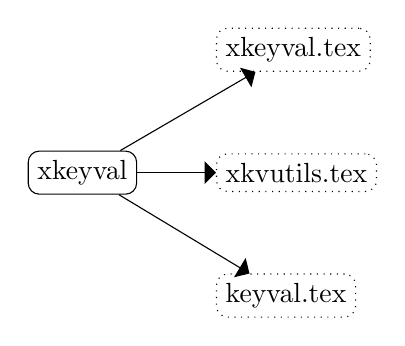
\begin{tikzpicture}
 \tikzset{main node/.style={rectangle, draw,
 		text centered, rounded corners}, }
 \tikzset{internal node/.style={rectangle, draw,dotted,
 		text centered, rounded corners}, }
 \tikzset{driver node/.style={ellipse, draw,dashed,
 		text centered}, }
 \tikzset{formato node/.style={rectangle, draw,dotted,
 		text centered}, }
 \tikzset{cfg node/.style={minimum size=1cm}, }
 \tikzset{linea/.style={-triangle 90},}
 \node[main node] (1) {xkeyval};
 \node[internal node] (3) [above right =of 1] {xkeyval.tex};
 \node[internal node] (4) [right =of 1] {xkvutils.tex};
 \node[internal node] (5) [below right =of 1] {keyval.tex};
 \foreach \x /\y in{1/3,1/4,1/5}
 \path[linea] (\x) edge node {} (\y);
 % 
 \end{tikzpicture}
\end{document}